No capítulo anterior, exploramos a análise de sentimento das postagens de eventos de zeladoria pública e a classificação das modelo de classificação baseado em aprendizagem de máquina; categorizamos os usuários em duas personas: "helpers" e "complainers". Os "helpers" são proativos, transmitindo mensagens construtivas e buscando colaborar para o bem-estar da comunidade. Em contraste, os "complainers" são mais críticos, frequentemente apontando falhas e expressando insatisfações. Além disso, capturamos o score de sentimento expresso nas postagens dos usuários em um modelo regressivo que varia de -1 para postagens com sentimento negativo e 1 para postagens com sentimento positivo. Neste capítulo, exploraremos como essas informações podem ser utilizadas para calcular a pressão social hiperlocal, com a intenção entender como as preocupações dos cidadãos se disseminam na rede e permitindo uma análise contextualizada dos discursos.

Cada postagem no Colab é mais do que uma simples expressão de sentimentos; ela está diretamente vinculada a eventos específicos de zeladoria pública, com tipos de eventos pré-definidos, que dão contexto ao conteúdo compartilhado. Estes tipos de evento de zeladoria podem variar desde preocupações com segurança, como "Ponto de tráfico de drogas", até perturbações como "Ponto recorrente de Poluição Sonora" ou questões ambientais como "Poda de Árvore". A combinação desses tipos de eventos, o score de sentimento das postagens e as personas classificadas e a localização do evento, oferece uma visão holística das interações dos cidadãos na plataforma, permitindo uma compreensão mais aprofundada das preocupações e necessidades da comunidade. Nesse sentido, podemos considerar o Colab como uma ferramenta inovadora para monitoramento e análise de sentimentos em tempo real, capturando a essência das preocupações e sentimentos dos cidadãos em reação a mudanças que ocorrem no ambiente urbano. Ao categorizar postagens por eventos específicos, a plataforma fornece insights valiosos para tomadores de decisão, pesquisadores e outros stakeholders. 

Portanto, consideramos que o Colab além de ser um aplicativo móvel, uma rede social de cidadania e uma empresa de GovTech, pode ser entendido também como o que viemos a chamar de "Barômetro Social Hiperlocal". Este conceito sugere que a plataforma não apenas capta as opiniões e sentimentos dos cidadãos, mas o faz levando em consideração as particularidades de diferentes localidades e temáticas. Assim, cada feedback fornecido pelos usuários pode ser interpretado como uma medida da "pressão" social de uma área ou tema específico. O termo "barômetro social" geralmente se refere à capacidade de medir a opinião pública. No entanto, ao adicionar "hiperlocal", estamos destacando a especificidade geográfica e temática das opiniões. O Colab exemplifica esse conceito, permitindo uma análise contextualizada dos discursos tanto em diferentes localidades quanto em variados assuntos. Autoridades, organizações e cidadãos podem se beneficiar dessa ferramenta, obtendo uma compreensão mais profunda das preocupações locais e adaptando suas ações e políticas de acordo. Aplicativos como o Colab não apenas fornecem uma plataforma para participação cidadã, mas também se estabelecem como um instrumento vital para a tomada de decisões informadas em uma sociedade cada vez mais conectada e dinâmica. Os usuários do Colab não apenas expressam seus sentimentos e opiniões sobre eventos de zeladoria pública, mas também o fazem de forma geolocalizada e categorizada por tipo de evento. Esta característica única da plataforma a diferencia de outras redes sociais, como o Twitter, onde a opinião média sobre um tópico específico pode ser mais difícil de discernir devido à falta de categorização e geolocalização.

Durante a classificação manual das postagens para análise de sentimento e personas conduzida no capítulo anterior, identificamos padrões relacionados a tipos de eventos e sentimentos dos usuários. Por exemplo, postagens relacionadas à gentrificação mostram preocupações com a valorização imobiliária. Alguns usuários tendem a criar eventos de zeladoria no Colab destacando uma preocupação com a valorização ou desvalorização dos seus imóveis. Outras postagens refletem tensões sobre a presença de pessoas em situação de rua, enquanto algumas destacam preocupações com poluição sonora ou gestão da vegetação urbana. Além disso, postagens sobre gestão de resíduos e qualidade do ar indicam uma crescente conscientização ambiental. Alguns usuários também tendem a incorporar discursos políticos ou fiscais reverberando debates sobre governança e prestação de contas que acontecem fora das redes. Essa diversidade de tópicos revela a riqueza de insights que o Colab oferece sobre a dinâmica social e as prioridades locais. Nossa análise revelou que as preocupações dos cidadãos são variadas e contextualmente dependentes. O Colab reflete e amplifica as vozes dos cidadãos em questões locais. A geolocalização das postagens é fundamental para entender as preocupações específicas de cada comunidade, reforçando o caráter único do Colab como um barômetro social hiperlocal.

A singularidade do Colab está concentrada, principalmente, na produção e consumo de conteúdo em eventos de zeladoria pública. Estas postagens, categorizadas por tipos específicos de eventos e enriquecidas com informações geolocalizadas, fotos, comentários e \textit{likes} já fornecem aos stakeholders, especialmente às agências governamentais, uma perspectiva clara das necessidades e preocupações das comunidades. No entanto, ao adicionar uma camada de análise de sentimento, essa perspectiva pode se tornar ainda mais valiosa. Por exemplo, em um cenário em que uma mudança significativa é implementada, como a troca de empresas de coleta de lixo em uma cidade. A partir da análise dos dados produzido pelas interações do Colab, os tomadores de decisão podem monitorar em tempo real se a polaridade das postagens relacionadas a coleta de lixo piorou ou melhorou após essa mudança, servindo como um indicador da eficácia da decisão.

Assim, nossa hipotese é que aplicativos como o Colab não são apenas plataformas de interação, mas também podem ser entendidos como "Barômetros Sociais Hiperlocais". Esta perspectiva pode refinar os dados brutos da rede em um instrumento de \textit{feedback-loop}, não apenas para a expressão cidadã, eficácia de determinadas políticas públicas de acordo com o sentimento dos usuários. Ao compreender e responder às demandas expressas no Colab, as agências governamentais têm a oportunidade de aprimorar suas ações e políticas, garantindo uma gestão mais alinhada às necessidades e sentimentos das comunidades urbanas.

Entender o Colab como um "Barômetro Social Hiperlocal" é informada e inspirada pelo conceito de Homogeneidade de Opiniões, conforme descrito por \citeonline{2023_Atiqi_BOOK}. A ideia de medir a pressão social de determinados assuntos ou temas nas comunidades da rede surgiu a partir da busca pela quantificação da homogeneidade de opiniões dos usuários.

\begin{citacao}
	"A more general concept defines echo chamber as the lack of information diversity a person is exposed with. The opinion does not necessarily have to be agreed by the person, but the type of opinions surrounding them should be homogeneous. A non-political example as suggested by Pentland is in the case of online trading (...) The lack of opinion diversity in this case is also considered as an echo chamber." \cite[p. 17]{2023_Atiqi_BOOK}.
\end{citacao}

A homogeneidade de opiniões, conforme definido pelo autor, é um indicador-chave de câmaras de eco. Ao analisar padrões nas postagens e nos sentimentos expressos pelos usuários, é possível discernir se uma opinião ou perspectiva está sendo predominantemente reforçada. Também é possível entender a distribuição de opiniões entre os relacionamentos dos usuários na rede, verificando se a opinião é compartilhada por um grupo de amigos ou se é amplamente aceita por toda a rede. Essas heurísticas são cruciais para identificar câmaras de eco e podem ser aplicadas para detectar e mitigar a polarização de opiniões.

Câmaras de eco têm o potencial de distorcer a percepção da realidade e intensificar a polarização de opiniões, o que pode influenciar decisões políticas e a percepção das necessidades da comunidade. O Colab, ao ser interpretado como um "Barômetro Social Hiperlocal", oferece uma fonte de dados para uma análise profunda das opiniões dos usuários, levando em conta sentimentos e personas. Esta análise pode revelar a homogeneidade de opiniões na rede, indicando se determinadas comunidades estão operando como câmaras de eco. A partir dessa perspectiva, os stakeholders têm a oportunidade de promover diálogos mais diversificados e formular políticas públicas mais alinhadas com as demandas da população.

A perspectiva do barômetro social no Colab não apenas destaca a polaridade e o sentimento das postagens, mas também revela padrões nas interações dos usuários. Por exemplo, ao avaliar postagens sobre "poda de árvores" em uma comunidade, é possível discernir se a maioria dos usuários são "helpers" ou "complainers" e qual é o sentimento predominante. Além disso, ao entender como as opiniões se agrupam e se propagam, podemos identificar pontos de influência na rede, locais onde intervenções podem ser mais impactantes para dissipar câmaras de eco e promover uma diversidade de opiniões.

Baseado nesse paradigma do Colab como um barômetro social, emergem heurísticas específicas que podem ser utilizadas tanto para quantificar a pressão social em comunidades hiperlocais quanto para detectar câmaras de eco. A pressão social, por sua vez, pode oferecer insights sobre a homogeneidade de opiniões na rede. Estas heurísticas, que serão detalhadas na próxima seção, fornecem uma estrutura robusta para entender a dinâmica das opiniões e sentimentos dos usuários, oferecendo insights valiosos para a análise e intervenção em contextos urbanos.

\section{Heurísticas para cálculo da Pressão Social Hiperlocal}

Nesta seção, abordaremos as heurísticas desenvolvidas para quantificar a pressão ou polaridade dos discursos nas postagens de eventos de zeladoria pública no Colab. Estas heurísticas, originadas de uma combinação de literatura existente e insights práticos, se tornaram cruciais para entender a opinião média de um grupo de usuários sobre eventos específicos de zeladoria pública. Elas são essenciais para medir a pressão social em comunidades hiperlocais, fornecendo insights valiosos para tomadores de decisão, pesquisadores e outros stakeholders interessados em compreender as complexas dinâmicas urbanas.

A relevância dessas heurísticas reside na sua capacidade de capturar a essência das opiniões dos cidadãos em contextos urbanos específicos. Ao analisar os tipos de eventos e as dinâmicas de participação cidadã na plataforma, podemos identificar tendências, preocupações e áreas de interesse, auxiliando na tomada de decisões informadas.

O conjunto de dados utilizado para esta análise foi meticulosamente compilado. Identificamos todos os usuários que fazem parte das comunidades da rede, conforme detalhado no \autoref{chapter:06_exploratory}, das cidades de Niterói, Santo André e Mesquita na rede Colab. Posteriormente, todas as postagens disponíveis desses usuários em eventos de zeladoria pública foram analisadas. Utilizamos o modelo de classificação descrito no \autoref{chapter:07_sentiment} para prever a persona do usuário e atribuir um score de sentimento a cada postagem. Esta metodologia nos permitiu obter insights sobre o comportamento dos usuários, como a expressão de suas opiniões e sentimentos. Adicionalmente, categorizamos os tipos de eventos associados a cada postagem.

\begin{table}[htbp]
	\centering
	\caption{Modelo de Dados para Análise de Pressão Social Hiperlocal}
	\begin{tabular}{ll}
		\toprule
		\textbf{Campo}    & \textbf{Descrição}                                  \\
		\midrule
		event\_id         & Identificador único do evento                       \\
		colab\_user\_id   & Identificador único do usuário do Colab             \\
		score             & Score de sentimento atribuído à postagem do usuário \\
		persona\_value    & Persona prevista para o usuário que fez a postagem  \\
		event\_type\_id   & Identificador único do tipo de evento               \\
		event\_type\_name & Nome descritivo do tipo de evento                   \\
		\bottomrule
	\end{tabular}
	\label{tab:modelo-dados-barometro}
\end{table}

Na \autoref{tab:modelo-dados-barometro}, cada linha representa uma postagem no Colab e inclui informações como o ID do evento, o ID do usuário do Colab, a pontuação de sentimento associada à postagem, a persona atribuída ao usuário que a fez, o ID do tipo de evento e o nome do tipo de evento relacionado. Esses dados formam a base essencial para nossas análises, permitindo-nos calcular a pressão social hiperlocal e compreender as dinâmicas das preocupações urbanas nessas comunidades específicas.

Com base neste modelo de dados, iniciamos o processo de filtragem e agregação. Primeiro, focamos nos membros ativos das comunidades identificadas na análise exploratória conduzida no \autoref{chapter:06_exploratory}. Em seguida, selecionamos tipos de eventos específicos, agrupados por tema, para nossa análise. Esta seleção foi guiada pela intenção de avaliar a pressão social hiperlocal em relação a preocupações específicas de zeladoria pública. A \autoref{tab:event_types_barometer} apresenta os tipos de eventos selecionados para esta análise.

Após a filtragem, calculamos duas métricas-chave para cada tipo de evento: a pontuação média de sentimento e a persona média. A primeira reflete o sentimento médio das postagens, enquanto a segunda representa a distribuição média das personas dos usuários. Essas métricas são calculadas para cada tipo de evento, permitindo-nos comparar e analisar as diferenças entre eles. A \autoref{tab:barometer_metrics} apresenta as métricas calculadas para cada tipo de evento.

A visualização da pressão social hiperlocal é apresentada através de um gráfico de radar, uma representação gráfica que permite analisar e comparar diversas variáveis em relação a um ponto central. O gráfico possui dois planos distintos: o plano de score e o plano de persona.

\begin{figure}[htb]
	\centering
	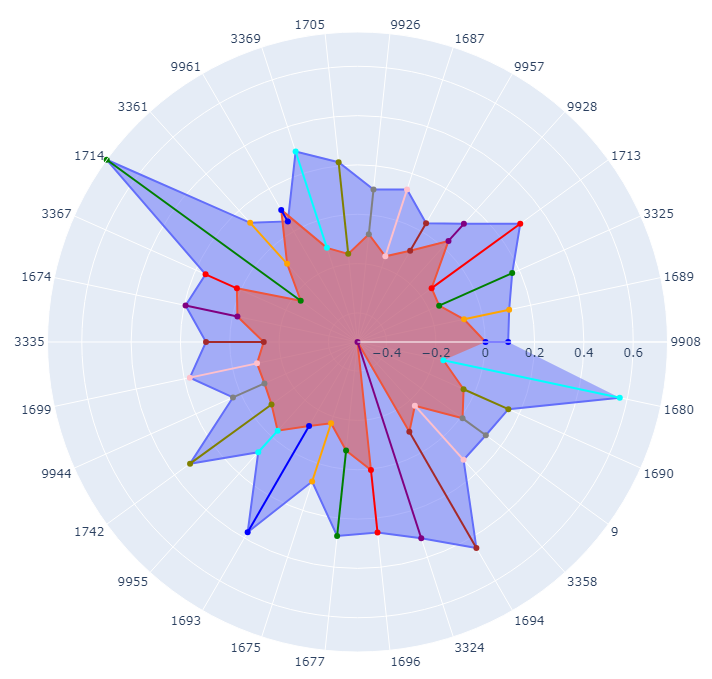
\includegraphics[width=0.7\textwidth]{images/social_barometer_plot.png}
	\caption{Gráfico de Radar para Análise de Pressão Social Hiperlocal. Os segmentos representam tipos de eventos, enquanto o eixo radial exibe valores médios de scores de sentimentos (plano vermelho) e personas (plano azul) atribuídos às postagens dos usuários relacionadas a cada tipo de evento.}
	\label{fig:social_barometer_plot}
\end{figure}

No plano de score, cada segmento do gráfico de radar representa um tipo específico de evento do Colab, onde cada evento é associado a um ângulo theta. O eixo radial, representado pelo parâmetro 'R', indica o valor médio dos scores de sentimentos atribuídos às postagens dos usuários em relação a um determinado tipo de evento. Quanto mais distante do centro estiver um segmento, maior será o valor médio do score e, consequentemente, mais positivo será o sentimento expresso pelos usuários em relação a esse evento. Por outro lado, segmentos mais próximos do centro indicam scores médios mais baixos, refletindo sentimentos mais negativos.

No plano de persona, novamente, cada segmento do gráfico representa um tipo de evento, O eixo radial 'R' neste caso indica o valor médio das personas previstas dos usuários em relação ao tipo de evento. Quanto mais próximo de 1 estiver um segmento, mais os usuários tendem a assumir uma persona de 'helper', caracterizada por atitudes positivas e colaborativas em relação ao evento. À medida que o valor de 'R' se aproxima de 0, os usuários tendem a adotar uma persona de 'complainer', indicando uma postura mais crítica e insatisfeita. Essa representação gráfica única proporciona uma visão abrangente e comparativa das opiniões e personas dos usuários do Colab em relação a diferentes tipos de eventos, permitindo uma análise mais profunda das dinâmicas das comunidades hiperlocais.

\subsection{Dinâmicas de Pressão Social nas Comunidades Colab}
A análise das interações no Colab revela uma rica dinâmica de participação cidadã em eventos de zeladoria pública. Com um total de 132.858 eventos registrados, observa-se uma participação ativa de 4.569 usuários únicos, indicando uma média de aproximadamente 29 eventos por usuário. Esta média sugere um engajamento considerável dos cidadãos na plataforma, refletindo sua preocupação e envolvimento ativo em questões de zeladoria em suas comunidades.

Ao explorar a estrutura de relacionamentos entre os usuários, identificamos 25.785 conexões, ou arestas, que delineiam a rede de interações no Colab. Estas arestas representam as conexões estabelecidas entre os 6.904 nós, ou entidades, que compõem a rede. Estes nós, em sua maioria, representam os usuários e suas características demográficas e geográficas.

Em relação à distribuição geográfica, Niterói emerge como a cidade com a maior representação, contabilizando 4.246 usuários. Em seguida, temos Santo André com 1.942 usuários e Mesquita com 716. No entanto, ao analisar a distribuição de eventos por cidade, observamos uma dinâmica interessante. Mesquita, apesar de ter o menor número de usuários, lidera em termos de eventos registrados, com um total de 63.927. Niterói, com o maior número de usuários, registra 42.191 eventos, enquanto Santo André contabiliza 26.740 eventos. Esta discrepância entre o número de usuários e o número de eventos sugere variações no nível de atividade e engajamento dos usuários em diferentes cidades.

A análise dos tipos de eventos reportados nas três cidades - Mesquita, Niterói e Santo André - revela padrões distintos de preocupações e demandas dos cidadãos em cada localidade, refletindo as particularidades e desafios urbanos enfrentados por cada comunidade.

Em Mesquita, o evento mais reportado, com uma expressiva quantidade de 45.235 registros, é "Entulho na calçada/via pública". Este número elevado sugere que a gestão de resíduos e a limpeza urbana são desafios significativos para a cidade. A presença massiva de entulho nas vias pode indicar problemas na coleta regular de lixo ou na conscientização da população sobre o descarte adequado. Além disso, eventos como "Bueiro entupido" e "Esgoto a céu aberto" também figuram no top 10, reforçando a ideia de que a infraestrutura urbana e os serviços de saneamento são áreas de preocupação para os cidadãos de Mesquita.

Por outro lado, em Niterói, a principal preocupação está relacionada à iluminação pública, com "Lâmpada apagada à noite" liderando a lista. Este tipo de evento, além de estar relacionado à segurança pública, também pode afetar a qualidade de vida dos cidadãos, uma vez que áreas mal iluminadas podem desencorajar atividades noturnas e a circulação de pessoas. Adicionalmente, "Buraco nas vias" e "Fiação irregular" também são frequentemente reportados, indicando possíveis desafios na manutenção das vias públicas e na infraestrutura elétrica da cidade.

Em Santo André, "Buraco nas vias" lidera as preocupações, seguido por eventos relacionados à gestão de resíduos e manutenção de áreas verdes, como "Entulho na calçada/via pública" e "Poda de árvore". Estes dados sugerem que, embora haja preocupações com a infraestrutura viária, também existe uma demanda significativa por espaços urbanos mais verdes e bem cuidados.

Estas variações nas principais preocupações reportadas em cada cidade refletem a diversidade de desafios urbanos enfrentados por diferentes comunidades. A pressão social, como medida pela frequência e tipo de eventos reportados, serve como um indicativo das áreas que requerem atenção prioritária das autoridades locais. Ao mesmo tempo, a capacidade dos cidadãos de reportar e categorizar eventos em plataformas como o Colab permite uma compreensão mais aprofundada das dinâmicas locais, oferecendo uma ferramenta valiosa para a tomada de decisões informadas.

Além disso, a análise desses eventos também pode fornecer insights sobre a eficácia das políticas públicas em vigor. Por exemplo, um aumento súbito no número de eventos relacionados a "Buraco nas vias" após uma temporada de chuvas pode indicar a necessidade de melhorias na infraestrutura viária. Da mesma forma, um número elevado de reportagens sobre "Entulho na calçada/via pública" pode sinalizar a necessidade de campanhas de conscientização sobre descarte adequado ou de melhorias nos serviços de coleta de resíduos.

\section{Polarização e Participação Cidadã no Ciberespaço}

A polarização, um fenômeno profundamente enraizado na psicologia social e política, encontrou um terreno fértil e amplificado na era digital. Estudos em análise de redes sociais têm destacado essa tendência. \citeonline{2020_Cossard}, por exemplo, delineia os grupos "pro-vacina" e "anti-vacina", enquanto \citeonline{2014_Colleoni} evidencia a divisão entre "Democratas" e "Republicanos" nas redes sociais. De forma intrigante, \citeonline{2018_Jasny} explora a polarização em contextos off-line, examinando o discurso de políticos sobre mudanças climáticas. Embora a pesquisa de \citeonline{2018_Jasny} não se concentre diretamente em ambientes online, suas observações sobre a polarização entre as abordagens "Binding Commitment", que propõem medidas mais conservadoras, e o "Clean Power Plan", que enfatiza a transição para energias limpas, ressoam com as dinâmicas observadas nas plataformas digitais.

\begin{figure}[htbp]
	\centering
	\begin{subfigure}{0.3\textwidth}
		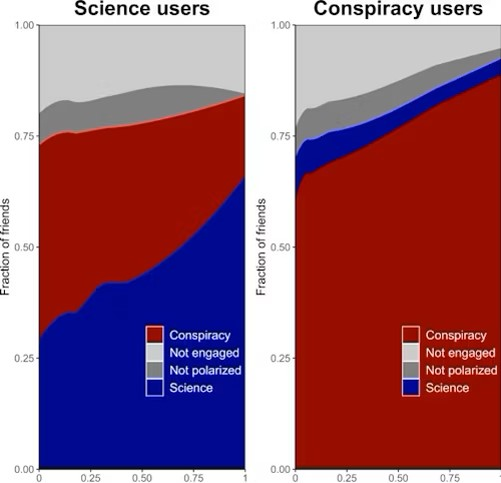
\includegraphics[width=\linewidth]{images/echo_chamber_graph_a.jpg}
		\caption{Gráfico demonstra câmara de eco entre usuários que seguem páginas de Ciência vs. Conspiraçao no Facebook e como nichos se afunilam promovendo isolamento entre usuários.}
		\fdireta{2019_Brugnoli}
		\label{fig:echo_chamber_graph_a}
	\end{subfigure}
	\hfill
	\begin{subfigure}{0.3\textwidth}
		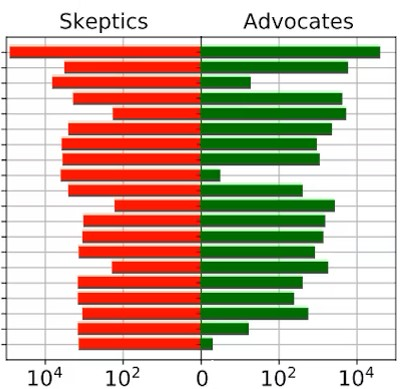
\includegraphics[width=\linewidth]{images/echo_chamber_graph_b.jpg}
		\caption{Gráfico demonstra a câmara de eco entre Céticos vs. Defensores da vacinação na Itália e como a polarização pode contribuir para a desinformação.}
		\fdireta{2020_Cossard}
		\label{fig:echo_chamber_graph_b}
	\end{subfigure}
	\hfill
	\begin{subfigure}{0.3\textwidth}
		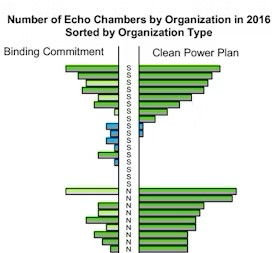
\includegraphics[width=\linewidth]{images/echo_chamber_graph_c.jpg}
		\caption{Grafico demonstra câmara de eco entre organicações no debate de políticas públicas de meio ambiente e mudanças climáticas dos EUA em 2016, especificamente sobre investir ou não em um plano de energia limpa.}
		\fdireta{2018_Jasny}
		\label{fig:echo_chamber_graph_c}
	\end{subfigure}
	\caption{Gráficos de polarização em estudos de análise de câmaras de eco.}
	\label{fig:echo_chamber_graph}
\end{figure}

Essa formação de grupos ideológicos não é meramente um reflexo da natureza humana, mas é intensificada pela arquitetura e algoritmos das plataformas digitais. Na busca por otimizar a experiência do usuário, essas plataformas frequentemente reforçam crenças preexistentes, gerando "bolhas de filtro", conforme observado por \citeonline{2016_Flaxman}. Essas bolhas, embora possam servir como escudos contra informações perturbadoras, também restringem a exposição a uma gama diversificada de perspectivas. No entanto, a era digital não se resume apenas a câmaras de eco. \citeonline{2019_Brugnoli} destaca que em ambientes online, mecanismos cognitivos, como a evitação de desafio, viés de confirmação, dissonância cognitiva e a busca por validação, são intensificados, com a validação frequentemente a um clique de distância. Essa noção, reforça papel das mídias sociais na formação e reforço dessas fenômenos no ciberespaço.

\begin{citacao}
	"Eu defino o ciberespaço como o espaço de comunicação aberto pela interconexão mundial dos computadores e das memórias dos computadores. Essa definição inclui o conjunto dos sistemas de comunicação eletrônicos (aí incluídos os conjuntos de redes hertzianas e telefônicas clássicas), na medida em que transmitem informações provenientes de fontes digitais ou destinadas à digitalização. Insisto na codificação digital, pois ela condiciona o caráter plástico, fluido, calculável com precisão e tratável em tempo real, hipertextual, interativo e, resumindo, virtual da informação que é, parece-me, a marca distintiva do ciberespaço" \cite[p. 102]{2010_Levy_BOOK}.
\end{citacao}

\citeonline{{2010_Levy_BOOK}}, por sua vez, argumenta que as dinâmicas "entrelaçadas" do ciberespaço refletem uma confluência de atores, projetos e interpretações, muitas vezes em oposição. O autor salienta que, apesar das tendências dominantes da era digital, a manifestação dessas tendências na vida cotidiana é multifacetada. A diversidade de interesses e perspectivas é emblemática da natureza fluida do ciberespaço. Enquanto alguns enxergam o ciberespaço como um domínio de comunicação livre e comunitária, outros o veem como um mercado global expansivo. Essas visões frequentemente colidem, ilustrando a complexidade e diversidade de vozes no ciberespaço. O autor também enfatiza que a representatividade cultural no ciberespaço é proporcional ao engajamento ativo e à qualidade das contribuições de seus participantes. Embora existam obstáculos à expressão da diversidade cultural, eles são menos proeminentes no ciberespaço do que em outros meios. Isso sugere que o ciberespaço, ao conectar indivíduos de diferentes origens, amplifica a diversidade de perspectivas. Em resumo, \citeonline{{2010_Levy_BOOK}} oferece uma perspectiva equilibrada e otimista sobre polarização e diversidade no ciberespaço. Ele reconhece os desafios da coexistência de múltiplas perspectivas, mas também vê o ciberespaço como um meio de expressão da diversidade cultural e colaboração. Isso sugere que, embora a polarização seja uma realidade, o ciberespaço também oferece oportunidades para diálogo e colaboração.

No contexto das plataformas digitais, a perspectiva de Lévy sobre a cibercultura é essencial para entender a dinâmica da polarização. Enquanto plataformas como o Colab podem enfrentar desafios de "bolhas de filtro" que limitam a diversidade de perspectivas, a natureza interconectada da cibercultura, conforme descrito por Lévy, também apresenta oportunidades. Essa interconexão pode facilitar diálogos construtivos e a negociação de diferentes pontos de vista. Portanto, ao reconhecer e valorizar essa diversidade, o Colab tem o potencial de se tornar um espaço inclusivo para o diálogo cidadão.A abordagem de Lévy sobre a cibercultura ressalta a natureza interconectada e a valorização da diversidade de perspectivas em discursos online evocam a utilização de heurísticas analíticas inovadoras que possam extrair informações estratégicas a partir dos dados de redes sociais. O Colab, além de ser um aplicativo e uma rede social de cidadania, pode ser classificado como um "barômetro social hiperlocal". Isso significa que, ao analisar postagens do ponto de vista de sentimentos e personas, é possível inferir a pressão social sobre determinados assuntos, relacionados a tipos específicos de eventos, de comunidades específicas em locais específicos. Assim, o "barômetro social hiperlocal" não é uma ferramenta separada, mas sim uma caracterização do próprio Colab e de sua capacidade de mediar e refletir as nuances das opiniões e sentimentos da comunidade.

Na análise sentimento e personas das postagens do usuários do Colab, uma tendência interessante se destaca: a maioria dos usuários foi classificado como 'helpers', com apenas alguns nichos dominados por 'complainers'. Esta classificação de personas proporciona entender de forma mais matizada da comunidade, destacando áreas de colaboração positiva e pontos de tensão. O conceito de 'barômetro social hiperlocal', aliado à análise de sentimentos das postagens, adiciona uma dimensão adicional ao nosso entendimento. Ao incorporar o tipo de evento como uma variável, podemos discernir nuances na pressão social manifestada pelos usuários. Enquanto, em média, as postagens tendem a adotar um tom mais neutro, a análise focada em eventos específicos revela áreas de intensa polarização, permitindo-nos identificar e abordar tópicos de particular tensão dentro da comunidade. Com as abordagens e ferramentas certas, como aquelas inspiradas por Lévy e implementadas no Colab, há um potencial significativo para promover a participação cidadã, o engajamento e a construção de comunidades mais informadas e coesas.